\hypertarget{grundzuxfcge-des-haftpflichtrechtes-gemuxe4ss-or-und-spezialgesetzen}{%
\section{Grundzüge des Haftpflichtrechtes gemäss OR und
Spezialgesetzen}\label{grundzuxfcge-des-haftpflichtrechtes-gemuxe4ss-or-und-spezialgesetzen}}

\hypertarget{werkeigentuxfcmerhaftpflicht}{%
\subsection{Werkeigentümerhaftpflicht}\label{werkeigentuxfcmerhaftpflicht}}

Ihrem Unternehmen gehört eine Lokalität im Herzen der Altstadt von
Liestal. Herr X, interessiert sich für Ihre Produkte, die er im
Schaufenster sieht und möchte Ihren Laden betreten. Er rutscht auf dem
Eis vor der Ausgangstüre aus und verletzt sich am Knöchel. Liegt hier
ein Fall der Werkeigentümerhaftpflicht vor? (Art. 58 OR)

\begin{itemize}
\tightlist
\item
  Schaden - Der Knöchel ging defekt, der Arzt kostet
\item
  Verschulden - Mangelhafte Unterhaltung des Werkes
\item
  Wiederrechtlichkeit - Unbetrittenes Recht für Gesundheit wurde
  verletzt
\item
  Werk: Alles, was künstlich hergestellt und mit dem Boden verbunden ist
\item
  Vorliegen eines Werkmangels: Werk bietet bei bestimmungsgemässen
  Gebrauch keine genügende Sicherheit
\item
  Kausalzusammenhang
\item
  Mangelnder Unterhalt
\item
  BGer: ``Wer den Besuchern eines Verkaufslokals eine Ausgangstüre zur
  Verfügung stellt, hat für deren möglichst gefahrlose Benützbarkeit zu
  sorgen. Dazu gehört auch, dass er unmittelbar jenseits der Türe
  laufende Gefahren, wie Glatteis auf dem Trottoir, im Rahmen des
  Möglichen und Zumutbaren beseitigt oder zumindest mit einem Warnschild
  (Achtung gschliferig) darauf aufmerksam macht.''
\end{itemize}

\hypertarget{produktehaftpflichtgesetz}{%
\subsection{Produktehaftpflichtgesetz}\label{produktehaftpflichtgesetz}}

\begin{figure}
\centering
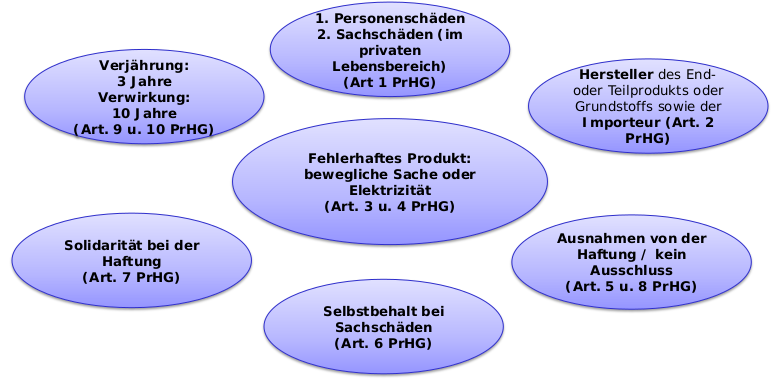
\includegraphics{figures/produkthaftpflicht.png}
\caption{Privathaftpflichtgesetz}
\end{figure}

\begin{itemize}
\tightlist
\item
  Der Schaden an Personen ist gedeckt
\item
  Private Sachschäden sind auch gedeckt. Werden jedoch Dinge von einem
  Unternehmen beschädigt, ist dies nicht gedeckt.
\item
  Produkthaftpflicht darf nicht durch AGBs oder andere Verträge
  ausgeschlossen werden
\item
  Solidarität bei der Haftung heisst: Auch wenn man als Importeur z.B.
  nichts für das Versagen des Produkts hat, haftet man und muss zahlen.
\item
  Die Produktehaftpflicht gilt nur 10 Jahre nach Einführung des Produkts
  und 3 Jahre nach Eintritt eines Schadens
\end{itemize}

\hypertarget{gefuxe4hrdungshaftung}{%
\subsection{Gefährdungshaftung}\label{gefuxe4hrdungshaftung}}

Die Gefährdungshaftung ist eine qualifizierte Kausalhaftung, indem sie
davon ausgeht, dass bestimmten Einrichtungen Gefahren inhärent sind, die
den Betreibern dieser Einrichtungen eine besondere Verantwortung
aufbürden.\\
BSP: Haftpflicht des Motorfahrzeughalters (SVG)

Art. 58.1 SVG

\begin{itemize}
\tightlist
\item
  Wird durch den Betrieb eines Motorfahrzeuges ein Mensch getötet oder
  verletzt oder Sachschaden verursacht, so haftet der Halter für den
  Schaden.
\end{itemize}

\hypertarget{voraussetzungen-haftpflichtrecht}{%
\subsection{Voraussetzungen
Haftpflichtrecht}\label{voraussetzungen-haftpflichtrecht}}

\begin{figure}
\centering
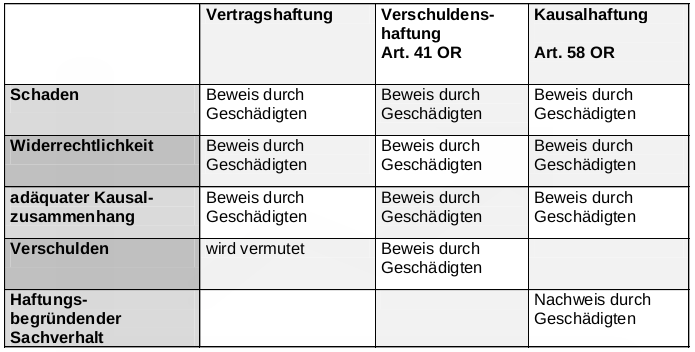
\includegraphics{figures/Voraussetzungen_Haftpflichtrecht.png}
\caption{Voraussetzungen Haftpflichtrecht}
\end{figure}

\hypertarget{culpa-in-contrahendo}{%
\subsection{Culpa in contrahendo}\label{culpa-in-contrahendo}}

Ist im Gesetz nirgends geregelt.

„Verschulden bei Vertragsverhandlung`` Voraussetzungen:

\begin{itemize}
\tightlist
\item
  es werden Verhandlungen über einen zukünftigen Vertrag geführt,
\item
  vorvertragliche Pflichten werden verletzt,
\item
  eine der Vertragsparteien erleidet einen Schaden, welcher
\item
  adäquat-kausal aus der Pflichtverletzung hervorgeht
\item
  und dem Verschulden der schädigenden Person zuzuschreiben ist.
\end{itemize}
